\documentclass[12pt]{article}

\usepackage{graphicx,color,enumerate,multicol}
\usepackage[top=1in, bottom=1in, left=1.25in, right=1.25in]{geometry}

%% Use Minion fonts if available.  Otherwise Times.
\IfFileExists{MinionPro.sty}{\usepackage[lf]{MinionPro}}{}
\usepackage{amsmath,amsthm,amsbsy}
\IfFileExists{MinionPro.sty}{}{\usepackage{times,txfonts}}

%% Setup aproblem environment, 
%% aproblem items
%% subproblems environment
%% subproblem items
\makeatletter
\newcounter{probcount}
\newcounter{subprobcount}
\newlength\probsep
\newlength\pshrinking
\newif\iffirstprob
\newenvironment{aproblems}%
  {\ifhmode\unskip\par\fi\setcounter{probcount}{0}\probsep\parskip
  \sbox\@tempboxa{\textbf{9.}}\pshrinking\wd\@tempboxa\advance\pshrinking\labelsep
  \let\hproblem\aproblem
  \advance\linewidth -\pshrinking
  \advance\@totalleftmargin\pshrinking
  \advance\leftskip\pshrinking}%
  {\ifhmode\unskip \par\fi\advance\leftskip-\pshrinking}%

\newcommand{\aproblem}{%
  \setcounter{subprobcount}{0}%
  \stepcounter{probcount}%
  \def\@currentlabel{\arabic{probcount}}%
  \ifhmode
    \unskip \par
  \fi
%  \addpenalty{-4000}%
  \iffirstprob\else\addvspace\probsep\fi
  \firstprobfalse
  \hskip -\labelwidth\hskip -\labelsep 
  \hbox to\labelwidth{\hss\textbf{\arabic{probcount}.}}\hskip\labelsep
}%

\newcommand{\subprob}{\item\def\@currentlabel{\arabic{probcount}\alph{\thelistlabel}}}
\newcommand{\skipproblem}{\stepcounter{probcount}}


%% The following commands put defined left and right headers on the top, and a page number
%% on the bottom of all pages beyond page 1
\usepackage{fancyhdr}
\pagestyle{fancy}
\fancyfoot[C]{\ifnum \value{page} > 1\relax\thepage\fi}
\fancyhead[L]{\ifx\@doclabel\@empty\else\@doclabel\fi}
\fancyhead[R]{\ifx\@docdate\@empty\else\@docdate\fi}
\headheight 15pt
\def\doclabel#1{\gdef\@doclabel{#1}}
\def\docdate#1{\gdef\@docdate{#1}}
\makeatother

%% General formatting parameters
\parindent 0pt
\parskip 6pt plus 1pt

\doclabel{Math F251: Section 2.1 Activity (Worksheet)}
\docdate{5 September 2018}

\begin{document}
%\renewcommand{\d}{\displaystyle}

\begin{aproblems}
\aproblem Here is a table of the temperature anomaly data, for recent years, from NASA.  I showed the whole 1880--2017 data set in class.  The first column is the year.  The second column is the difference of the globally-averaged temperature for that year minus the average of the 1951--1980 period, in Celsius.  The plot below shows this data.

\bigskip
\hspace{-15mm}\begin{minipage}[b]{0.4\textwidth}
\footnotesize
\begin{verbatim}
        1990        0.44
        1991        0.41
        1992        0.22
        1993        0.24
        1994        0.31
        1995        0.44
        1996        0.33
        1997        0.47
        1998        0.62
        1999         0.4
        2000         0.4
        2001        0.54
        2002        0.62
        2003        0.61
        2004        0.53
        2005        0.67
        2006        0.62
        2007        0.64
        2008        0.52
        2009        0.63
        2010         0.7
        2011        0.57
        2012        0.61
        2013        0.64
        2014        0.73
        2015        0.86
        2016        0.99
        2017         0.9
\end{verbatim}
\end{minipage}
\begin{minipage}[b]{0.6\textwidth}
\qquad 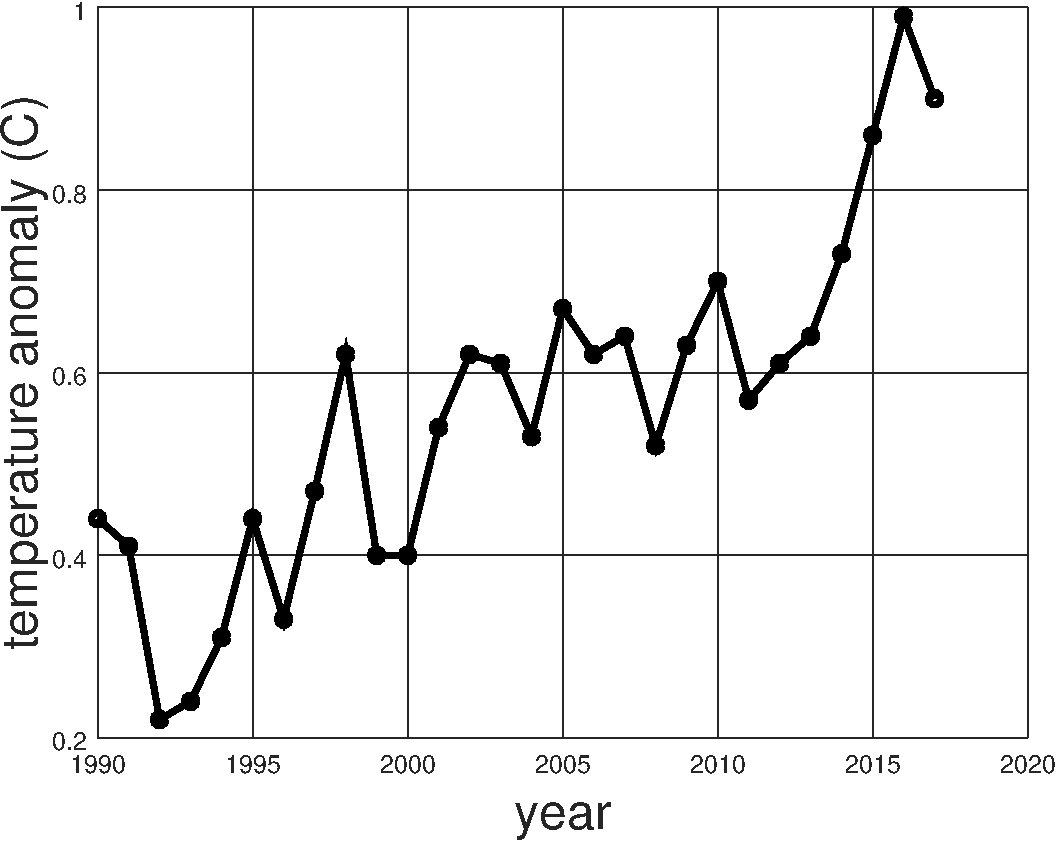
\includegraphics[width=0.95\textwidth]{recentyeartemp}
\end{minipage}

\normalsize
Compute from the data:

\vspace{-5mm}
\begin{enumerate}
\item the average rate of change of temperature (i.e.~slope of the secant line) in the period 1990--2017

\bigskip
\item the highest average rate of change you can compute for a ten-year period

\bigskip
\item the lowest rate of change you can compute for a ten-year period

\bigskip
\item your estimate of the rate of change in the year 2010
\end{enumerate}

\vfill
\footnotesize
\emph{This example shows that slopes can always be computed, \emph{but} that noisy data does not really have a slope when you look at a small period.  See the next page for better-behaved functions.  Math 251 Calculus I will be \emph{entirely} about well-behaved functions.  You see, Calc I is not real life.}
\vfill

\clearpage \newpage
\aproblem  (\emph{This is Exercise 3 in section 2.1}.)  The point $P(2,-1)$ lies on the curve $y=1/(1-x)$.
\renewcommand{\labelenumi}{\alph{enumi})}
\begin{enumerate}
\item Pick a point on the curve $(x,1/(1-x))$, not too far from $P$, and call it $Q$.  Sketch the curve, the points $P$ and $Q$, and the secant line $PQ$.
\item Use your calculator to find the slope of the secant line $PQ$ correct to six decimal places, for the following values of $x$:
    $$\begin{matrix}
    \text{(i) 1.5} & \text{(ii) 1.9} & \text{(iii) 1.99} & \text{(iv) 1.999} \\
    \\
    \text{(v) 2.5} & \text{(vi) 2.1} & \text{(vii) 2.01} & \text{(viii) 2.001}
    \end{matrix}$$
\item Using the results of part a), guess the value of the slope of the tangent line to the curve at $P(2,-1)$.
\item Find an equation for the same tangent line as in c).
\end{enumerate}
\vfill

\aproblem  (\emph{This is Exercise 2 in section 2.1.  Compare the nice result here to problem on the previous page}.)  A cardiac monitor is used to measure the heart rate of a patient after surgery.  It compiles the number of heartbeats after $t$ minutes, as in the table below.  When the data are graphed, the slope of the tangent line represents the heart rate in beats per minute.

\begin{tabular}{l|c|c|c|c|c}
$t$ (min) & 36 & 38 & 40 & 42 & 44 \\ \hline
heartbeats & 2530 &2661 & 2806 & 2948 & 3080
\end{tabular}

The monitor estimates the heart rate using secant line slopes.  Use the data to estimate the patient's heart rate at $42$ minutes using the secant line between the points
\renewcommand{\labelenumi}{\alph{enumi})}
\begin{enumerate}
\item $t=36$ and $t=42$
\item $t=38$ and $t=42$
\item $t=40$ and $t=42$
\item $t=42$ and $t=44$
\end{enumerate}
Give an (estimated) conclusion about the patient's heartbeat at 42 minutes.
\vfill


\end{aproblems}

\end{document}